\documentclass[
  manuscript=article,  %% article (default), rescience, data, software, proceedings, poster
  layout=preprint,  %% preprint (for submission) or publish (for publisher only)
  year=20xx,
  volume=x,
]{joas}
\usepackage{makecell}
\doi{xx.xxxxx/joas.xxxx.xxxx}

% \conference{} command is only used for proceedings
\conference{Conference Title}

\received {1 April 20xx}
\revised  {1 May 20xx}
\accepted {10 May 20xx}
\published{20 May 20xx}

\editor{Editor Name}

\reviewers{First Reviewer, Second Reviewer, Third Reviewer}

% specify the .bib file for references
\addbibresource{reference-joas.bib}

% --- below is the area for authors ---

% Title within 12 words
\title{Evaluating the Impact of ADS-B Data Cleaning on Algorithm Performance}

\author{Ruolan REN}
\affiliation{Civil Aviation University of China, Tianjin, China}
\email{rowanren@qq.com}



\author{Jingcheng ZHONG}
\affiliation{Civil Aviation University of China, Tianjin, China}


\author{Dizhi GUO}
\affiliation{Civil Aviation University of China, Tianjin, China}

\author{Ruixin WANG \orcid{0000-0002-3585-2524}}
\affiliation{Civil Aviation University of China, Tianjin, China}
\email{ruixin.wang@recherche.enac.fr}


\author{Christophe HURTER \orcid{0000-0003-4318-6717}}
\affiliation{Université de Toulouse, ENAC, Toulouse, France}
\affiliation{ IPAL Singapore, Singapore}
\email{christophe.hurter@recherche.enac.fr}

% maximum five keywords
\keywords{ADS-B Data; Data Cleaning; Data Quality; Algorithm Performance}

% Important: don't overuse abbreviations. Only use abbreviations if the term is used more than ten times throughout the paper. Otherwise, write them in full.
\abbreviations{
    JOAS: Journal of Open Aviation Science, % remove this in your paper!
    ATM: Air Traffic Management % remove this in your paper!
}

\begin{document}
\begin{abstract}
  Automatic Dependent Surveillance-Broadcast (ADS-B) data have become a key resource for research on trajectory prediction, conflict detection, and air traffic management. However, due to inherent limitations in data acquisition and transmission, ADS-B datasets often contain missing points, irregular sampling, and anomalies. To ensure usability, researchers typically perform data cleaning and preprocessing before analysis. While these operations improve consistency and completeness, they inevitably alter the original data characteristics, potentially causing deviations between algorithm outputs and actual operational patterns. Existing studies tend to focus on specific cleaning methods, but lack systematic and quantitative evaluations of how different cleaning strategies impact downstream applications. To address this gap, this paper proposes an indicator-driven, structured evaluation framework. The framework integrates a multi-level data quality metric system, datasets with varying levels of cleaning, and comparative experiments under a unified prediction and analysis setup to examine how data cleaning influences algorithm performance. Experimental results demonstrate that differences in cleaning strategies can substantially affect prediction accuracy and reliability, highlighting the importance of balancing data cleaning and fidelity. This study provides a systematic approach for evaluating ADS-B data quality and establishes a more robust data foundation for trajectory prediction, safety assessment, and air traffic management applications.
\end{abstract}

\section{Introduction}

ADS-B has become a crucial data source for air traffic management, supporting a wide range of applications. Typical studies include trajectory prediction~\cite{wang2021performance,corrado2021clustering}, flight phase identification~\cite{schlosser2024analysis}, trajectory clustering and modeling~\cite{guleriamachine}, safety analysis~\cite{noh2018aviation} (e.g., conflict detection and collision risk assessment), and airport operations optimization~\cite{roosenbrand2023contrail} (e.g., runway occupancy and taxiing analysis). ADS-B has also become a key enabler for environmental studies such as fuel consumption estimation, contrail detection, and large-scale emissions assessment.
Despite these advances, ADS-B data quality remains a significant concern. Missing points, irregular sampling, and anomalies complicate processing and may bias analysis. To improve usability, researchers apply cleaning methods such as interpolation, smoothing, outlier removal, and resampling. However, these methods can also distort the statistical and physical characteristics of trajectories. For example, interpolation can mask subtle variations and increase prediction errors, while outlier removal may discard rare but genuine safety-critical events. Yet, existing studies rarely provide systematic and quantitative analysis of how different strategies influence downstream results.
To address this gap, this study systematically evaluates the relationship between data cleaning and algorithmic performance in ADS-B analytics. Chapter \ref{soa} reviews eight major application domains of ADS-B data to contextualize its analytical value. Chapter \ref{clean}  summarizes common data cleaning techniques and proposes a generalized preprocessing pipeline integrating detection, interpolation, and smoothing. Chapter \ref{usecase} presents an autoencoder-based case study that quantifies the impact of different noise types (Gaussian, drift, and spikes) on trajectory reconstruction performance, followed by a discussion of the observed impacts and implications. Finally, Chapter \ref{conclusion} concludes the study and outlines directions for future research. These analyses aim to provide a clearer understanding of how data quality shapes learning-based ADS-B algorithms and to inform the design of more robust data processing strategies.
\section{State of the Art}

This chapter provides a systematic review of ADS-B technology and its current applications in aviation research. It begins with a review of the development and technical evolution of the ADS-B system, highlighting its role and advantages within modern air traffic management. Subsequently, based on a systematic literature review, the use of ADS-B data across different research domains is summarized and categorized, outlining the main directions and emerging trends. This overview lays the theoretical and practical foundation for the subsequent chapters on data cleaning and algorithm performance evaluation.


\subsection{ADS-B History}
In the early stages of civil aviation, air traffic controllers primarily relied on Primary Surveillance Radar (PSR) and Secondary Surveillance Radar (SSR) to monitor aircraft. However, with improvements in aircraft performance and the expansion of long-haul air routes, the limitations of PSR and SSR—such as restricted coverage, insufficient information accuracy, and delayed updates—gradually became apparent. These limitations not only increased the navigational difficulty for long-distance flights but also posed safety risks. For instance, in 1983, Korean Air Flight 007 deviated from its intended route due to insufficient radar coverage, navigation system malfunctions, and communication failures~\cite{icao_1993}, ultimately entering Soviet airspace and being shot down, resulting in a major aviation accident.

To address these challenges, the aviation industry gradually developed the Automatic Dependent Surveillance–Broadcast (ADS-B) system over several decades. ADS-B leverages the Global Navigation Satellite System (GNSS) and onboard sensors, integrating information such as barometric altitude, inertial navigation, and airspeed measurements to generate aircraft state parameters. These parameters, including identification codes, position, altitude, velocity, and flight intent, are periodically broadcast via onboard ADS-B equipment~\cite{olive2024filtering}. Compared with traditional radar, ADS-B offers higher accuracy, shorter update intervals, broader coverage, and lower infrastructure and maintenance costs. It significantly enhances situational awareness for both pilots and air traffic controllers while reducing the burden on ground surveillance infrastructure.

The development of ADS-B can be traced back to the 1970s. In 1992, the Radio Technical Commission for Aeronautics (RTCA) first proposed ADS-related technical specifications in DO-212~\cite{RCTA_DO-212}, identifying it as a candidate technology for future air traffic surveillance. The DO-242 standard~\cite{RCTA_DO-242} issued in 1998 further established the technical framework and performance requirements for ADS-B systems. Between 1996 and 2006, the Federal Aviation Administration (FAA) conducted the CAPSTONE project in Alaska~\cite{faa2000capstone}, demonstrating the potential of ADS-B to improve operational safety and efficiency in remote airspace. In 2003, the 11th Air Navigation Conference of the International Civil Aviation Organization (ICAO) formally recognized ADS-B as a critical surveillance technology for future air traffic management and promoted its standardization and adoption~\cite{icao_2003}.

Since 2010, ADS-B has gradually entered large-scale global deployment. Various countries have promoted its adoption through regulations. The FAA requires all aircraft operating in controlled airspace to be equipped with ADS-B Out~\cite{cfr91-225}; Europe has similarly mandated ADS-B under the SESAR framework~\cite{undertaking2009european}, expecting to increase European airspace capacity by 80–100\% by 2040. Australia~\cite{casa2010cao20-18} and Singapore have also implemented ADS-B mandates. In China, a national policy issued in 2015~\cite{caac2015adsb} required the installation of ADS-B equipment on commercial aircraft. Meanwhile, satellite-based ADS-B~\cite{melero2024satera} has enabled real-time and high-precision surveillance over approximately 70\% of global airspace, and open platforms such as the OpenSky Network~\cite{schafer2014bringing} provide large-scale ADS-B data resources for academic research.


\subsection{ADS-B Data current usages}

This section presents an overview of the current use of ADS-B data in the research domain, identifying and organizing clusters of algorithms and application areas. In this study, the collected literature is categorized into eight major domains, spanning from trajectory modeling and operational management to environmental sustainability and cybersecurity. These analyses provide a structured overview of the evolving research landscape surrounding ADS-B applications in aviation.

 \subsubsection{Paper Selection}

This section describes the process of identifying, screening, and organizing research publications related to the application of ADS-B data. To ensure both representativeness and research quality, we focused on journals and conferences with high academic impact in the fields of air traffic management (ATM) and digital aviation. The primary sources include the \textit{Digital Avionics Systems Conference (DASC)}, \textit{SESAR Joint Undertaking Annual Conference}, \textit{Air Traffic Management Seminar (ATM Seminar)}, \textit{International Conference on Research in Air Transportation (ICRAT)}, \textit{Transportation Research Part C: Emerging Technologies}, \textit{IEEE Transactions on Intelligent Transportation Systems}, and the \textit{Journal of Air Transport Management (JATM)}. Literature retrieval was mainly conducted through academic databases such as IEEE Xplore, ScienceDirect, and Elsevier Scopus, as well as publicly available proceedings from the aforementioned conferences.

Considering that large-scale implementation and operational use of ADS-B systems began worldwide around 2012, this year was set as the starting point for the large-scale research phase of ADS-B data. Therefore, this study selected English-language publications issued between 2012 and December 2024 as the objects of analysis. We manually collected research that explicitly utilized real ADS-B flight data from the selected journals and conferences, excluding studies that relied solely on simulated or synthetic datasets.

The detailed screening process was as follows:

\begin{itemize}
    \item \textbf{Initial Screening:} Titles and abstracts were reviewed to confirm the study’s relevance to the aviation domain, such as airspace optimization, trajectory prediction, or conflict detection and avoidance (DAA).
    \item \textbf{Keyword Filtering:} Only papers containing the term ``ADS-B'' in the title, abstract, or keywords were retained.
    \item \textbf{Data Authenticity Criterion:} Studies were required to clearly indicate the use of real ADS-B datasets. Papers using only simulated or artificially generated trajectories were excluded.
    \item \textbf{Duplication and Accessibility Review:} Duplicate publications and inaccessible preprints were removed to ensure the reproducibility and verifiability of the results.
\end{itemize}

After multiple rounds of screening and manual verification, a total of 145 papers were collected, covering representative applications of ADS-B data across diverse research domains. The distribution of the selected studies by source is illustrated in Figure ~\ref{fig:placeholder}.

\begin{figure}
    \centering
    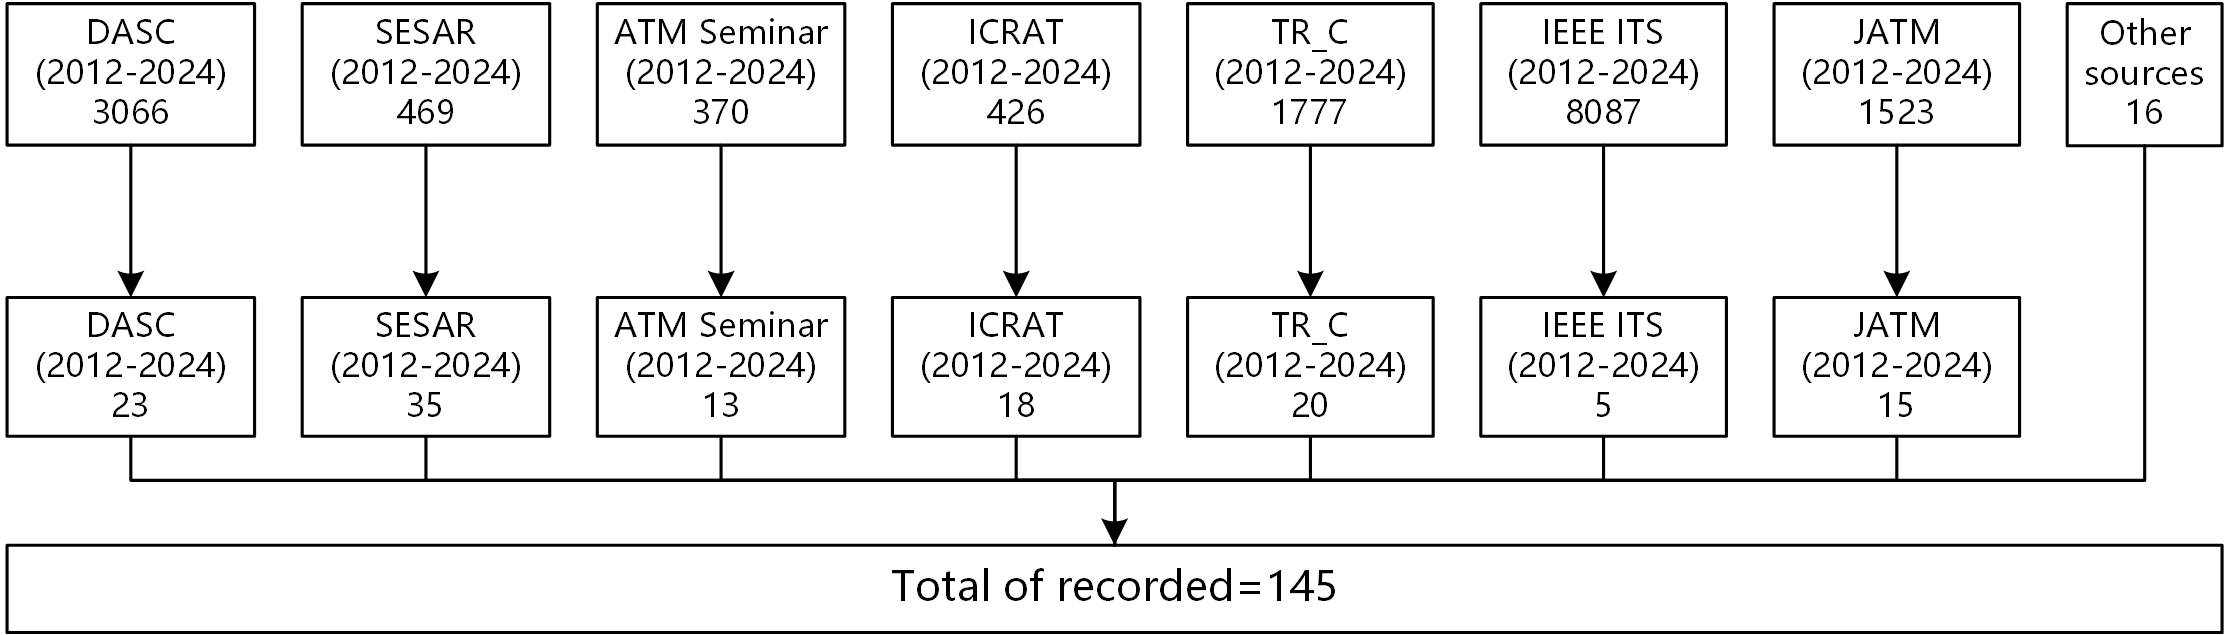
\includegraphics[width=1\linewidth]{paper_selection1.png}
    \caption{Paper collection flow}
    \label{fig:placeholder}
\end{figure}
\subsubsection{Paper Clustering and Categorization}

The screened publications provided a solid data foundation for the categorization and trend analysis of ADS-B applications in this study. To systematically organize the characteristics and focal points of different research directions, we employed a mixed quantitative–qualitative approach for feature extraction and clustering of the collected literature.

Using Excel spreadsheets and reference management tools, the following key features were extracted from each selected conference and journal:
\begin{itemize}
    \item Publication year;
    \item Source conference or journal;
    \item Paper title and author keywords;
    \item Application scenario;
    \item Research focus or analytical perspective;
    \item Methods and algorithmic approaches (e.g., machine learning, optimization models, statistical analysis, simulation frameworks);
    \item Description of the ADS-B dataset used (e.g., public data repositories, airport-specific data, or crowdsourced datasets).
\end{itemize}

In the preliminary organization stage, the literature was grouped into four broad directions: trajectory prediction, air traffic management, aircraft performance estimation, and environmental sustainability. However, a subsequent systematic comparison and semantic analysis of all research features revealed significant overlaps and hierarchical relationships among different themes.

Therefore, this study adopted a combination of thematic synthesis and semantic grouping to reclassify the literature. This process comprehensively considered the research objectives, data utilization patterns, and the functional role of ADS-B within each study, aiming to establish a classification framework that systematically reflects the overall landscape of ADS-B research.

Finally, ADS-B–related studies were categorized into eight major domains:
Trajectory Modeling and Prediction, Operational Optimization and Management, Operational Safety and Surveillance, Aircraft Performance and Efficiency, Data Engineering and Enhancement, Environment and Sustainability, Security and Cybersecurity, Methodology, Simulation, and Policy.
This classification framework provides the structural foundation for the domain-specific analysis presented in the following sections.

As shown in Table \ref{tb: 8categories}, the classification results derived from thematic induction and semantic grouping are presented, covering typical application domains of ADS-B data across eight research categories and their representative algorithms. In the following sections, each category is further elaborated in terms of its research scope and representative studies.



\begin{table}[h]
	\centering
	\caption{Summary of ADS-B Application Categories, Main Methods, and Data Roles}
	\label{tb: 8categories}
	\begin{tabular}{p{3cm} p{6cm} p{3cm}}
		\hline
		\textbf{Category} & \textbf{Main Methods} & \textbf{Role of ADS-B Data} \\
		\hline
		\textbf{Trajectory Modeling and Prediction} &
		\makecell[l]{Clustering (DBSCAN, K-means)\\
			LSTM/Transformer prediction\\
			Autoencoder feature extraction\\
			DTW\\
			PCA\\
			Hybrid physical–data models} &
		\textbf{Core data source} \\
		\hline
		
		\textbf{Operational Optimization and Management} &
		\makecell[l]{
			MILP\\
			Simulated annealing\\
			Heuristic algorithms\\
			KPI-based performance metrics\\
			Historical traffic analysis
		} &
		\textbf{Real-time/historical traffic input} \\
		\hline
		
		\textbf{Operational Safety and Surveillance} &
		\makecell[l]{
			DAA geometric models\\
			Anomaly detection (thresholds, clustering, autoencoder, GMM)\\
			Monte Carlo risk evaluation
		} &
		\textbf{Flight monitoring and safety baseline} \\
		\hline
		
		\textbf{Aircraft Performance and Efficiency} &
		\makecell[l]{
			Dynamic equation inversion\\
			Maximum likelihood estimation\\
			Bayesian inference\\
			Particle filtering\\
			Regression and neural networks
		} &
		\textbf{Model calibration data source} \\
		\hline
		
		\textbf{Data Engineering and Enhancement} &
		\makecell[l]{
			Kalman filtering\\
			Map-matching\\
			Multisource fusion\\
			Data indexing\\
			Generative models (TimeGAN)
		} &
		\textbf{Primary processing object} \\
		\hline
		
		\textbf{Environment and Sustainability} &
		\makecell[l]{
			Trajectory-based emission estimation\\
			Remote sensing data fusion\\
			Optimal control route planning
		} &
		\textbf{Environmental assessment input} \\
		\hline
		
		\textbf{Security and Cybersecurity} &
		\makecell[l]{
			Intrusion detection (ML classifiers)\\
			Protocol vulnerability testing\\
			SDR signal analysis
		} &
		\textbf{Research target} \\
		\hline
		
		\textbf{Methodology, Simulation, and Policy} &
		\makecell[l]{
			Open-source simulation platform development\\
			Data standardization\\
			Policy and privacy analysis
		} &
		\textbf{Research infrastructure and policy object} \\
		\hline
	\end{tabular}
	\label{tab:adsb_applications}
\end{table}

\textbf{Trajectory Modeling and Prediction.} 
This domain focuses on modeling historical and real-time aircraft trajectories and predicting their future states. The core tasks include 4D prediction, estimated time of arrival (ETA) calculation, trajectory pattern clustering and quantification of prediction uncertainty. As the core data source, ADS-B provides continuous, high-precision measurements of aircraft position, velocity, and altitude, forming the foundation for trajectory modeling and prediction. The data quality directly affects model accuracy and reliability. Gui et al. \cite{xuhao2021trajectory} proposed a semantic trajectory representation for arrival flight clustering to support airspace design, flow management, and ETA estimation; Wang et al. \cite{wang2017short} applied PCA-based dimensionality reduction and DBSCAN clustering for preprocessing, followed by a Multi-Cell Neural Network (MCNN) for short-term trajectory prediction in terminal maneuvering areas (TMA); and Wang et al. \cite{wang2018hybrid} integrated clustering-based preprocessing with hybrid MCNN models to improve ETA prediction accuracy.

\textbf{Operational Optimization and Management.} 
This domain focuses on improving the overall efficiency of airspace and airport operations, encompassing air traffic flow management, surface operations (taxiing and sequencing), terminal maneuvering area coordination, and airspace structure optimization. ADS-B data play a central role by providing continuous and fine-grained historical and real-time traffic information, serving as a reliable input for optimization models and decision-support systems. It enables accurate operational performance evaluation and data-driven strategy optimization. Research in this area often applies Linear Programming, Simulated Annealing, and heuristic algorithms to address sequencing, scheduling, and routing problems. Other studies employ queuing models and Key Performance Indicators (KPIs) for operational assessment or mine historical ADS-B data to identify bottlenecks such as taxiway congestion and sector capacity limits. Basora et al. \cite{basora2018occupancy} combined DBSCAN clustering with Random Forest regression for sector occupancy prediction, and Delahaye et al. \cite{delahaye2022air} used hierarchical clustering with Transformer models for flow pattern detection and capacity management.

\textbf{Operational Safety and Surveillance.} 
This research domain aims to enhance aviation safety and situational awareness through data-driven analysis. It covers conflict detection and resolution (DAA / ACAS), abnormal event detection (e.g., go-arounds, unstable approaches), assessment of collision risk and airspace complexity, and performance evaluation of surveillance systems. As an independent surveillance source, ADS-B data provide continuous and high-precision trajectory and state information, enabling real-time monitoring of aircraft behavior, detection of potential conflicts and anomalies, and quantitative assessment of operational safety.
Bonifazi et al. \cite{bonifazi2021modeling} identified unstable approaches and go-arounds using ADS-B data, employing rule-based methods and Gaussian Mixture Models (GMM) for anomaly detection and integrating runway and weather information for improved accuracy. Rorie et al. \cite{rorie2024detect} conducted the first real-world evaluation of the ACAS Xr airborne collision avoidance system. Zhang et al. \cite{zhang2024study} investigated conflict-free routing strategies and compared multiple optimization algorithms, while Bao et al. \cite{bao2024exploring} proposed a multi-airport terminal area risk prediction framework to assess inter-airport conflict probabilities. 

\textbf{Aircraft Performance and Efficiency.} 
This research area focuses on deriving aircraft performance parameters from flight data to calibrate or complement existing models such as BADA, and to evaluate energy efficiency across aircraft types and flight phases. Key parameters include aircraft mass, drag polar, thrust settings, fuel consumption, and speed profiles.
In this context, ADS-B data provide essential flight state information—such as ground speed, vertical rate, and heading—enabling large-scale, fleet-level performance analysis even in the absence of detailed design data. This supports more accurate and data-driven model calibration and validation.
Sun et al. \cite{sun2018aircraft} developed a probabilistic framework to estimate aerodynamic parameters from operational data; Schultz et al. \cite{schultz2022data} integrated FDR and ADS-B data to model fuel consumption and operational efficiency using machine learning methods; and Alligier et al. \cite{alligier2020predictive} predicted aircraft mass and speed intent during climb to enhance physics-based trajectory prediction.

\textbf{Data Engineering and Enhancement.} 
This category focuses on improving the quality and usability of raw ADS-B data, which form the foundation for subsequent analytical and modeling applications. Key tasks include data cleaning and anomaly detection, missing-value imputation, multi-source data fusion, data compression and indexing, and synthetic data generation. In this domain, ADS-B data themselves are the core subject of engineering—aimed at producing cleaner, more complete, and more interoperable datasets that support trajectory prediction, operational analysis, and safety evaluation.
Tabassum et al. \cite{tabassum2017ads} conducted long-term statistical analysis to identify anomalies and assess the impact of systematic errors on trajectory accuracy. Wandelt et al. \cite{wandelt2018ads} introduced an efficient compression and indexing framework to enable scalable querying and analytics of large-scale ADS-B records. Spinielli et al. \cite{spinielli2017initial} developed a reproducible reference trajectory dataset by integrating multiple surveillance sources for performance assessment under the EUROCONTROL PRU initiative.

\textbf{Environment and Sustainability.}
This research area focuses on quantifying the environmental impact of aviation operations and exploring sustainable optimization strategies, including greenhouse gas and pollutant emission assessment, contrail formation detection and avoidance, and noise evaluation. Owing to its wide coverage and high temporal resolution, ADS-B data serve as a crucial source for environmental modeling and validation. For instance, Roosenbrand et al. \cite{roosenbrand2023contrail} proposed a method to estimate contrail altitudes using shadows in Landsat satellite imagery, with ADS-B data employed as ground truth for validation. Sun et al. \cite{sun2023evaluating} integrated satellite-based and ground-based ADS-B data with wind field information to improve emission estimation and compared actual flight trajectories with optimal routes to quantify excess emissions.

\textbf{Security and Cybersecurity.}
This domain focuses on identifying and mitigating cybersecurity threats targeting the ADS-B system itself, such as False Data Injection Attacks (FDIA), signal spoofing, and message tampering, to ensure the integrity and reliability of surveillance information. In this field, the ADS-B protocol, signal, and data link are the direct subjects of vulnerability analysis and protection technology research. For example, Cretin et al.\cite{cretin2018increasing} proposed a Domain-Specific Language (DSL)-based testing framework to evaluate the resilience of Air Traffic Control (ATC) systems against FDIA, while Khan et al. \cite{khan2021intrusion} employed machine learning techniques for ADS-B intrusion detection.

\textbf{Methodology, Simulation, and Policy.}
This category provides foundational tools, frameworks, and policy support for aviation research. It includes the development of open-source simulation platforms, advocacy of reproducible research practices, establishment of data standards, and discussion of regulatory and privacy issues related to ADS-B deployment. In this context, ADS-B serves both as input data for constructing realistic scenarios in simulation environments and as a focal topic in advancing data-sharing policies, privacy protection, and industry standards. For example, Mehlitz et al. \cite{mehlitz2019analyzing} proposed the RACE framework for comprehensive airspace data analysis, while Bolic et al. ~\cite{bolic2024roadmap} systematically elaborated on the European ATM Open Science Alliance and its Open Performance Data Initiative (OPDI), which aim to foster transparency and open research in the ATM domain.

To provide a clearer overview of the application fields of ADS-B data, we conducted a quantitative analysis of field attribution for 145 valid papers from journals including DASC and SESAR, based on the eight aforementioned classification categories. The results are presented in Figure \ref{fig:paperpiechart2}. It should be noted that some papers cover multiple fields (e.g., Data Engineering + Aircraft Performance Calculation) and are assigned to multiple application fields in accordance with the rule of "counting each involved field separately". Consequently, the total number of papers counted in the pie chart is greater than the actually counted 145 valid samples.

From the overall distribution, papers related to Operational Optimization and Management represent the most prominent field in ADS-B data research, accounting for 30.6\%. This is followed by Operational Safety and Surveillance (23.6\%) and Trajectory Modeling and Prediction (18.5\%). These three fields collectively account for over 70\% of the total, forming the mainstream directions of ADS-B data applications. This reflects a high alignment between ADS-B data-related research and the core application scenarios of ADS-B: Operational Optimization and Management directly addresses the efficiency needs of air traffic management (ATM) systems, such as "improving airspace utilization and reducing flight delays"; meanwhile, Operational Safety and Surveillance, as well as Trajectory Modeling and Prediction, leverage the "real-time positioning and dynamic tracking" capabilities of ADS-B to serve the safety requirements of "flight conflict early warning and rapid identification of abnormal states".

In contrast, the proportions of papers in the fields of Security and Cybersecurity (2.5\%), Environment and Sustainability (5.1\%), and Methodology, Simulation and Policy (5.1\%) are relatively low, collectively accounting for less than 15\%. These fields represent the directions with relatively smaller proportions in current ADS-B data application research.

% TODO: \usepackage{graphicx} required
\begin{figure}
	\centering
	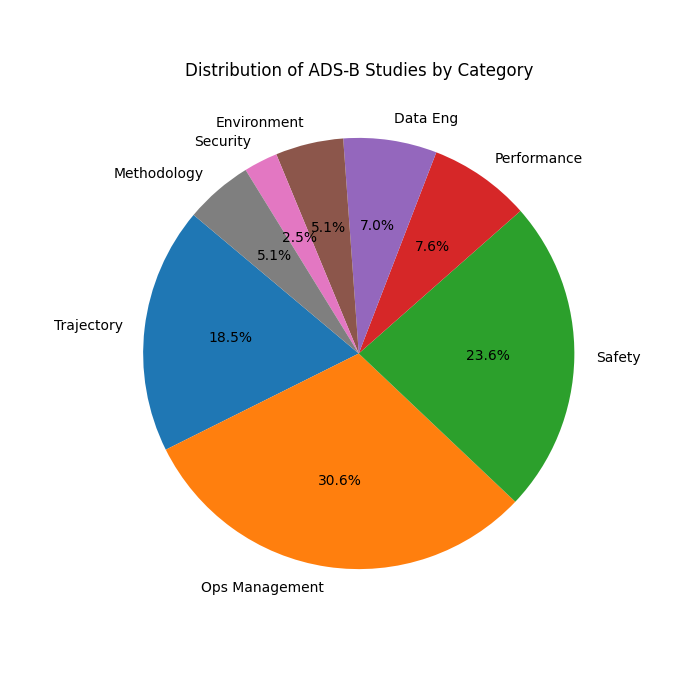
\includegraphics[width=0.5\linewidth]{paper_piechart}
	\caption[Figure 2]{Distribution of studies across 8 ADS-B application domains}
	\label{fig:paperpiechart2}
\end{figure}


 %\subsection{ADSB Data future usages}
\section{Summary of ADSB Cleaning Methods, work flow}

Advantages/mandatory cleaning process

Pro:

Correct the data, remove errors, make the data coherent

 cons

Data distortion,
Data uncertainty,
Data error injections
Inject non existing data (e.g. new data)


Mitigation plan:

how to find the right balance between data cleaning and data accuracy



\section{Algorihtm Robustness}
\section{Conclusion}


This paper will present the design of an evaluation framework and its application to ADS-B data. 
The framework is intended to provide researchers and practitioners with practical tools to select appropriate cleaning strategies, 
balance data fidelity with usability, and build more reliable foundations for trajectory prediction, safety assessment, and air traffic management. 
In addition, the paper will contribute:
\begin{itemize}
  \item an overview of the current use of ADS-B data in the research domain, identifying and structuring clusters of algorithms in use;
  \item an analysis of the main trends in ADS-B data usage based on a systematic literature review;
  \item extraction of a representative set of algorithms that rely on ADS-B data and testing their robustness under varying data correction strategies; and
  \item conclusions on algorithm sensitivity to data cleaning, with a discussion of trade-offs between preprocessing, fidelity to original data, and downstream accuracy, as well as future research directions.
\end{itemize}



%\section{Abstract Extension}

With the rapid growth of global air traffic, traditional radar surveillance systems, such as primary surveillance radar (PSR) and secondary surveillance radar (SSR), have shown increasing limitations in coverage, accuracy, and cost. To address these issues, ADS-B technology was developed. Relying on satellite navigation and onboard sensors, ADS-B uses the Global Navigation Satellite System (GNSS) to obtain position and velocity information, which is then integrated with barometric altitude, inertial navigation, and airspeed measurements to generate flight state data. This information is periodically broadcast via ADS-B devices, including identifiers, position, altitude, velocity, and flight intent~\cite{olive2024filtering}. Compared with traditional radar, ADS-B significantly enhances situational awareness for both pilots and air traffic controllers, while reducing infrastructure construction and maintenance costs.

The development of ADS-B can be traced back to the 1970s, with its concept first proposed and later validated in the U.S. FAA’s Safe Flight 21 project during the 1990s. The “Capstone Program” in Alaska (1999-2006)~\cite{faa2000capstone} further demonstrated its ability to improve safety and efficiency in remote airspace. In 2003, the 11th ICAO Air Navigation Conference officially recognized ADS-B as a surveillance method and promoted standardization. Since the 2010s, ADS-B has entered large-scale deployment: the U.S. FAA mandated “ADS-B Out”~\cite{cfr91-225}, Europe implemented ADS-B under the SESAR framework~\cite{undertaking2009european}, and Australia~\cite{casa2010cao20-18}, Singapore, and other countries followed suit, with China issuing its national implementation plan in 2015~\cite{caac2015adsb}. More recently, space-based ADS-B technology~\cite{melero2024satera} has extended global coverage, while open platforms such as OpenSky Network~\cite{schafer2014bringing} have improved data accessibility and research value.

Beyond surveillance, ADS-B data are widely used in both research and operational applications. Typical studies include trajectory prediction ~\cite{wang2017short}\cite {yoon2023improving}, flight phase identification~\cite{wang2021performance}, trajectory clustering and modeling~\cite{corrado2021clustering}, safety analysis~\cite{schlosser2024analysis} (e.g., conflict detection and collision risk assessment), and airport operations optimization~\cite{guleriamachine} (e.g., runway occupancy and taxiing analysis). ADS-B is also applied in environmental studies, such as fuel consumption estimation~\cite{noh2018aviation}, contrail detection~\cite{roosenbrand2023contrail}, and large-scale emissions assessment~\cite{sun2023evaluating}.


Despite its widespread use, ADS-B data quality remains a significant concern. Limitations in acquisition and transmission often result in missing points, irregular sampling, and anomalies, which increase processing difficulty and may bias analysis results. To enhance usability, researchers typically apply data cleaning and preprocessing methods, such as time-series interpolation, trajectory smoothing, outlier removal, and resampling. While these methods improve data completeness and consistency, they can alter the statistical and physical characteristics of the original trajectories, potentially affecting downstream algorithms. For example, interpolation can fill missing points and improve completeness, but excessive interpolation may smooth subtle variations, increasing trajectory prediction errors. Outlier removal enhances physical plausibility but may discard extreme but genuine events, causing missed warnings in conflict detection or safety assessment. Trajectory smoothing reduces position jitter but weakens turning or curvature features, affecting behavior-based prediction or identification models. Resampling standardizes sampling intervals for easier model processing but may introduce artificial speed or vertical rate changes, impacting time-dependent prediction algorithms. These examples illustrate the complex and conditional impact of data cleaning on algorithm performance. Existing studies generally focus on data-level improvements and lack systematic, quantitative analysis of how different cleaning strategies affect downstream algorithm outputs. Therefore, it is necessary to construct multi-level data quality metrics, create datasets of varying quality, and conduct controlled experiments under a unified algorithm framework to elucidate the role of data cleaning in ADS-B applications and provide methodological support for trajectory prediction, safety assessment, and air traffic management.

To address this need, this article develops a structured and indicator-driven evaluation framework. By quantifying data quality across multiple dimensions, generating datasets of different quality levels, and performing comparative experiments under a unified algorithmic environment, the framework enables a quantitative assessment of how various cleaning strategies affect algorithm performance.

In the data quality evaluation stage, a multi-dimensional metric system was designed to quantify data quality from different perspectives. For example, completeness measures the alignment between observed points and theoretical sampling frequency, approaching 1 when deviations are below a set threshold and the time series is continuous. Reliability reflects the physical plausibility of flight trajectories, approaching 1 when speed, climb rate, and other parameters are within reasonable ranges. Consistency captures spatial and temporal smoothness and continuity. Further analysis indicates that different metrics exhibit varying sensitivity to algorithm performance: completeness strongly affects predictive and analytical results, while some physical constraints have a limited impact. Understanding metric sensitivity not only helps explain algorithm performance differences but also informs more precise data cleaning strategies.

In dataset construction, high-quality, carefully cleaned trajectories were used as an “ideal” reference, with controlled anomalies (e.g., random noise, missing points, trajectory perturbations, and resampling) introduced to create datasets of varying quality. This design ensures comparability in experiments while simulating the diversity and complexity of real-world data, providing a realistic basis for algorithm evaluation.

In the algorithm validation stage, datasets of varying quality were fed into a unified set of application algorithms (e.g., trajectory prediction or air traffic management models). Comparative analysis across datasets quantifies the effect of data cleaning and quality differences on algorithm performance. This approach clarifies the role of data processing in ADS-B applications and supports the reliability and reproducibility of related algorithms.

By integrating a multidimensional evaluation system with a structured experimental framework, this study not only reveals the specific impacts of different data cleaning strategies on algorithm performance, but also clarifies the sensitivity of various data quality metrics, providing a quantitative assessment method and a robust data foundation for trajectory prediction, safety assessment, and air traffic management applications.

%Large comment to skip this
\iffalse
\section{User guide for this template}

\textcolor{red}{DO NOT submit papers containing LaTeX error messages.} If you see any error messages, please fix them before submission. Please read the following guidelines carefully.

The copy editor is Junzi alone for the moment; any time saved for him is time saved for you :).

\subsection{Title}
The title should be in Title Case. Keep it concise and informative, ideally within 12 words. Avoid abbreviations in the title unless they are widely recognized.

\subsection{Single main file}
\textcolor{red}{DO NOT use external .tex files}, like \verb|\input{}| or \verb|\include{}|. Place all content in \texttt{main.tex}.

\subsection{Keep the original file names}
\textcolor{red}{DO NOT rename filenames} including \texttt{main.tex}, the \texttt{figures} folder, or \texttt{reference.bib}, to ensure compatibility with the automated copyediting process.

\subsection{References}
Add your bibliography entries to \texttt{reference.bib} and cite them using \verb|\cite{}|. Here is an example citation on diamond open access \cite{fuchs2013diamond}. Since many of you are using the OpenSky data, here is another example \cite{schafer2014bringing}.

\subsection{Footnotes}
Use footnotes sparingly. They should be used for additional information that is not essential to the main text. Use the \verb|\footnote{}| command to create footnotes.\footnote{This is an example footnote that works.}

\subsection{Tables}
Use the standard \texttt{tabular} environment. \textcolor{red}{Avoid custom or complex table designs} to ensure compatibility for the web version. Table \ref{tb:example_table} shows an example that always works.

\begin{table}[htbp!]
  \centering
  \small
  \caption{Example table}
  \label{tb:example_table}
  \begin{tabular}{lll}
  \toprule
  \textbf{Parameter} & \textbf{Notation} & \textbf{Remarks} \\
  \midrule
  name & - & engine common identifier \\
  manufacture & - & name of the manufacturer  \\
  bpr & $\lambda$ & bypass ratio \\
  pr & - & pressure ratio \\
  thrust & $T_0$ & maximum static thrust\\
  \bottomrule
  \end{tabular}
\end{table}

\subsection{Figures}
Store all figures in the \textbf{figures} folder. Use concise, space-free, and lowercase filenames.

Ensure that the figure is in a compatible format (.png or .pdf) and is appropriately sized (not too large or too small). Figure~\ref{fig:example} shows an example of how to include a figure.

\begin{figure}[htbp!]
  \centering
  \includegraphics[width=0.4\textwidth]{example-image}
  \caption{An Example Figure}
  \label{fig:example}
\end{figure}

If you need subfigures, \textcolor{red}{DO NOT use the \texttt{subfloat} package}. You are recommended to use the \texttt{subfigure} package instead. Figure~\ref{fig:subfig_example} shows an example of how to use subfigures.

\begin{figure}[htbp!]
  \centering
  \subfigure[First subfigure]{\includegraphics[width=0.3\textwidth]{example-image-a}}
  \hspace{0.2cm}
  \subfigure[Second subfigure]{\includegraphics[width=0.3\textwidth]{example-image-b}}
  \caption{An Example of subfigures}
  \label{fig:subfig_example}
\end{figure}

Attention: in your text, use \verb|Figure \ref{fig:example}|, NOT \verb|Fig. \ref{fig:example}|.


\subsection{Equations}
Use the \verb|equation| environment for numbered equations. You must avoid customized variable names. Otherwise, the HTML version will not be generated properly.

For example, Equation \ref{eq:cauchy_momentum} shows an example equation.

\begin{equation} \label{eq:cauchy_momentum}
\rho\frac{\mathrm{D} \mathbf{u}}{\mathrm{D} t} = - \nabla p + \nabla \cdot \boldsymbol \tau + \rho\,\mathbf{g}
\end{equation}

\subsection{Abbreviations}
Use the \verb|\abbreviations{}| command to define abbreviations. Only use abbreviations if the term is used more than ten times throughout the paper. Otherwise, write them in full.


\section{Sections}

Organize your paper using standard sectioning commands (\verb|\section|, \verb|\subsection|, etc.).

Some standard sections are:

\begin{itemize}
  \item Introduction
  \item Methods
  \item Results
  \item Discussion
  \item Conclusion
\end{itemize}

You can add or remove sections as needed.

Use \verb|Appendix| for supplementary material. The appendix should be used for additional information that is not essential to the main text but may be useful for some readers. Remove this section if you do not have any supplementary material.

\appendix

\section{Supplementary figures}

\section{Supplementary tables}


\section*{Acknowledgement}
Include your acknowledgements in this section.

% Author contributions (CRediT) are mandatory for all papers with more than one author
\section*{Author contributions}
If the paper has more than one author, the CRediT section must be included. See example usage at \url{https://casrai.org/credit/}

\begin{itemize}
  \item First Author: Conceptualization, Data Curation, Formal Analysis, Funding Acquisition, Investigation, Methodology, Project Administration, Resources, Software, Supervision, Validation, Visualization, Writing (Original Draft), Writing (Review and Editing)
  \item Second Author: Data Curation, Writing - Original Draft
  \item Third Author: Visualization, Investigation
\end{itemize}


\section*{Funding statement}
When applicable, please specify the funding information for this research.


% Data statement is mandatory for all papers
\section*{Open data statement}
\textcolor{red}{Mandatory section!}

Include DOI and a short description of supplementary data.

% reproducibility statement is mandatory for all papers
\section*{Reproducibility statement}
\textcolor{red}{Mandatory section!}

Information on how to reproduce this research, including access to: 1) source code related to the research, 2) source code for the figures, 3) source code/data for the tables when applicable.

%end large comment
\fi

%\input{introduction.tex}

%\input{SoA.tex}
%\input{christophe.tex}

%\input{ADSBCleaning.tex}

%\input{AlgortihmRobustness}


\printbibliography
\end{document}